\subsection{Anforderungsspezifikation}

\subsubsection{Funktionale Anforderungen}

\subsubsection{Nicht-Funktionale Anforderungen}
Beim Thema Nicht-Funktionale Anforderungen halten wir uns an die Standards ISO 9126\cite{ISO9126} bzw. dessen Nachfolger ISO 25010\cite{ISO9126_ISO25010}. Beide ISO-Normen sind sich sehr ähnlich und liefern eine gute Checkliste für jegliche Art von Systemanforderungen.

\begin{figure}[h]
	\centering
	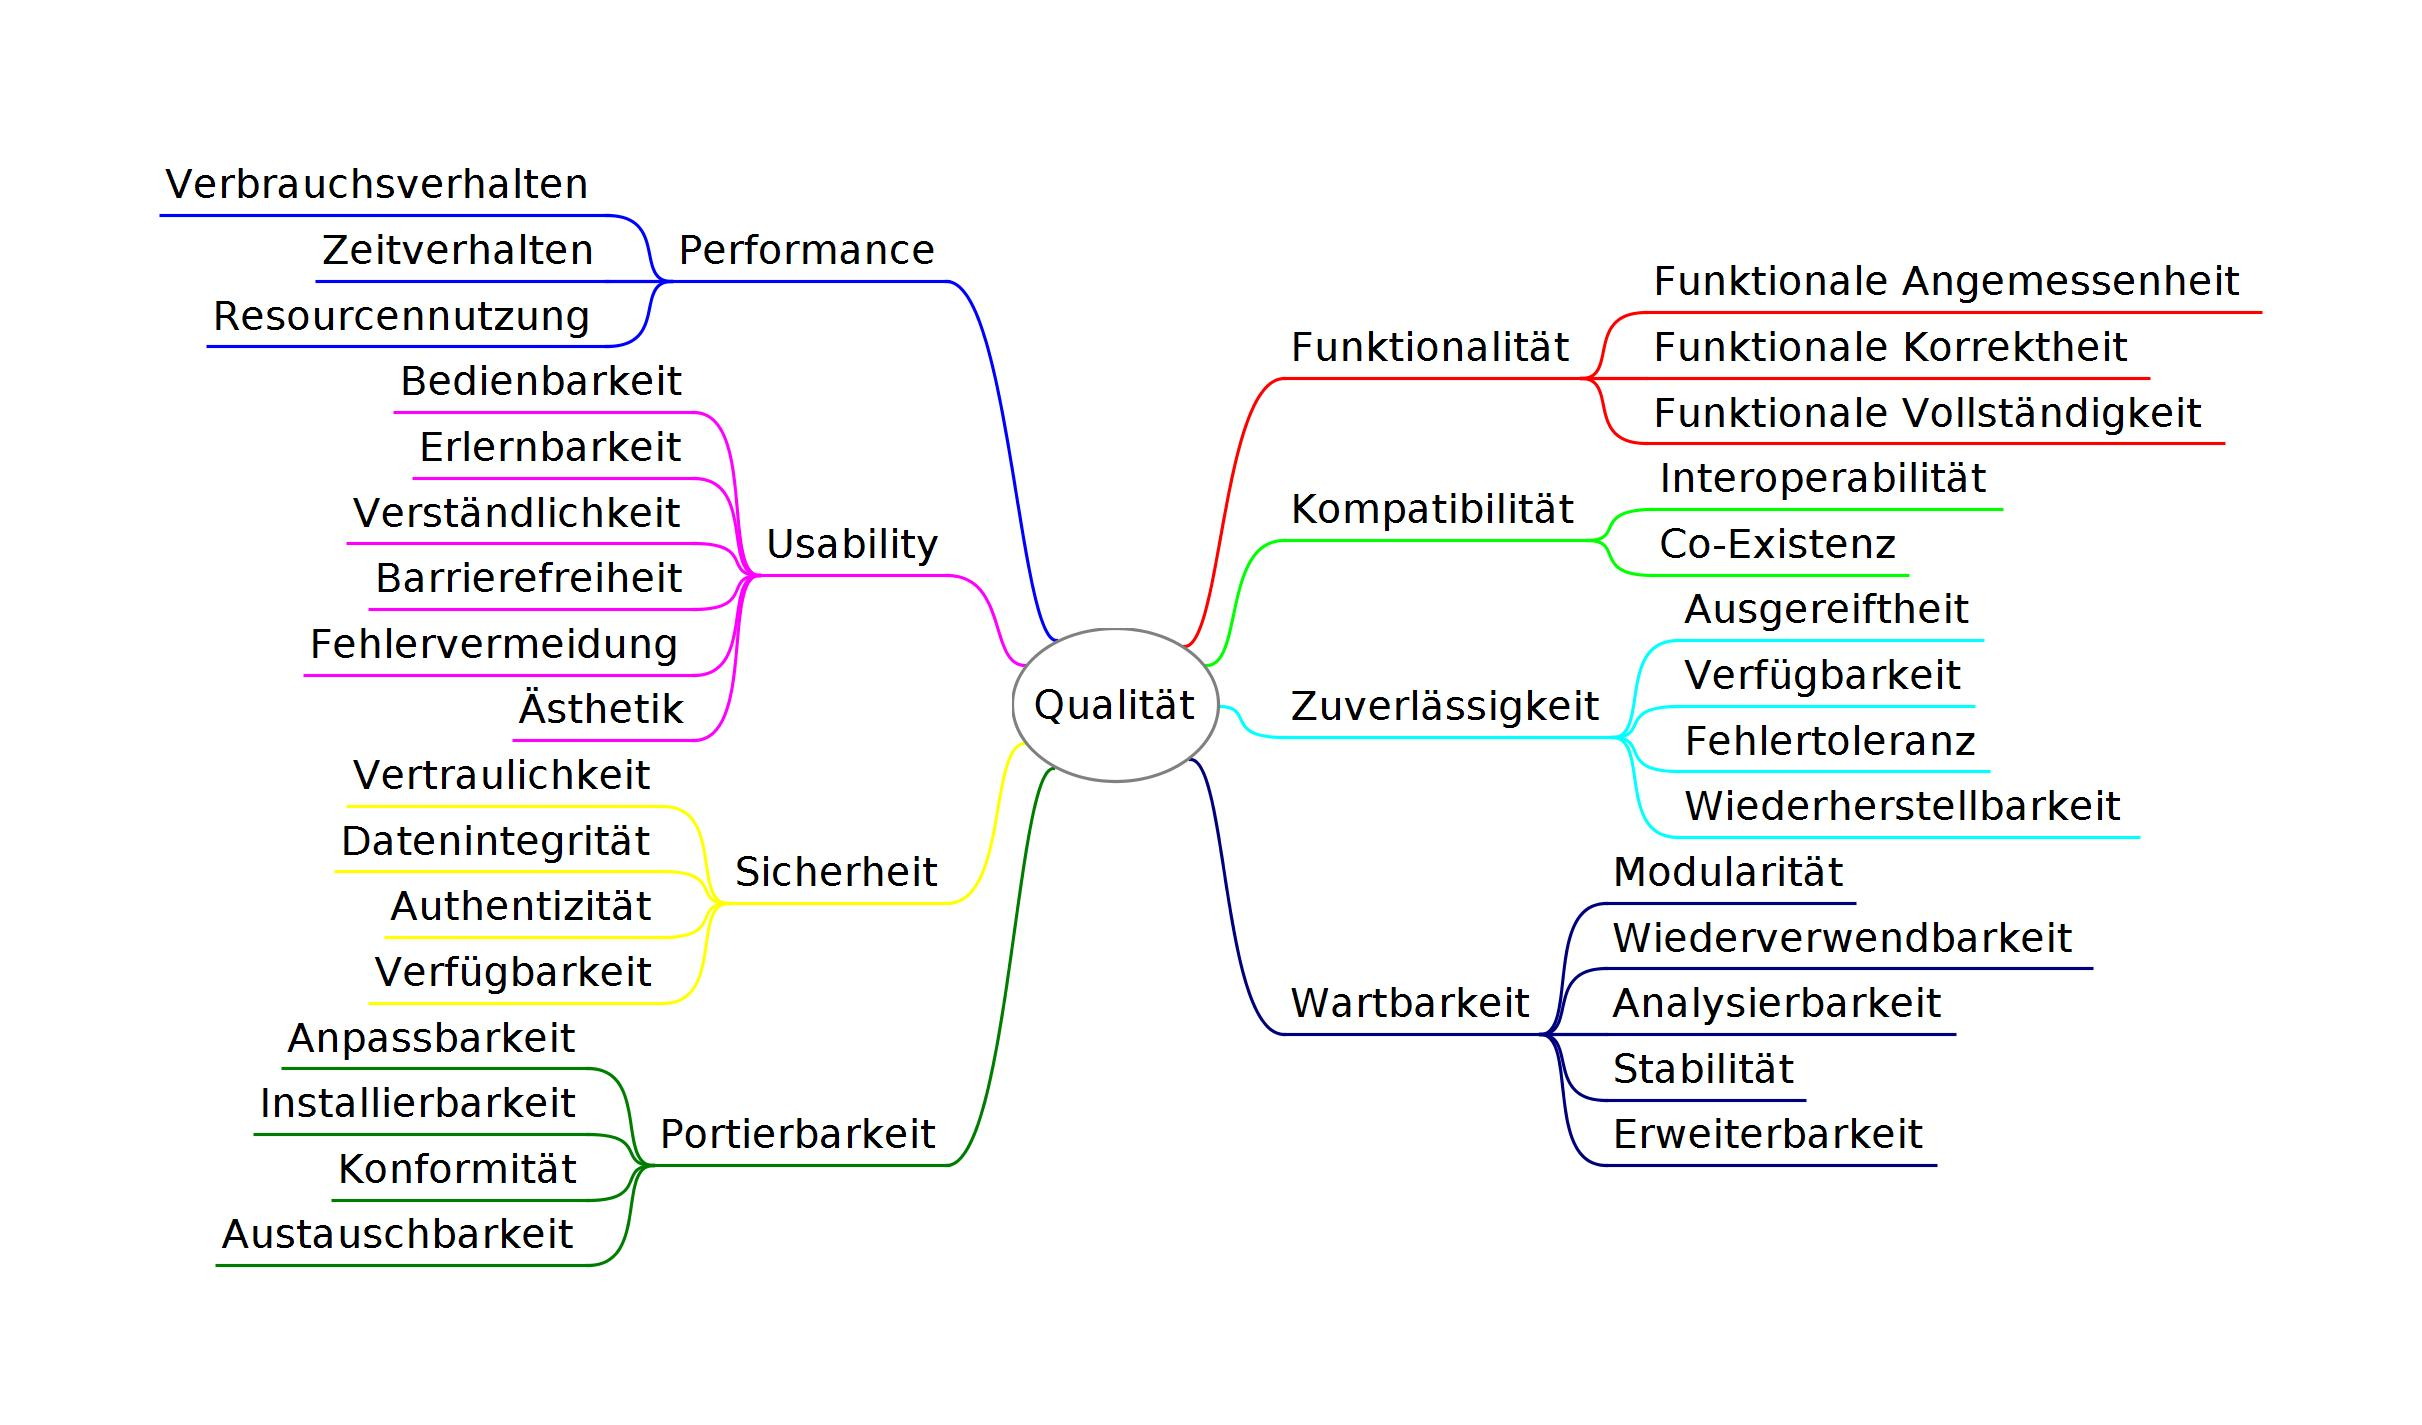
\includegraphics[width=1\linewidth]{img/anforderungen/quality}
	\caption[Anforderungskategorien nach ISO 25010]{Anforderungskategorien nach  ISO 25010}
	\label{fig:ISO 25010}
\end{figure}

%TODO Bild Link: https://blog.seibert-media.net/blog/2018/05/14/qualitaet-funktionale-und-nichtfunktionale-anforderungen-in-der-software-entwicklung/

Diese Normen sind sehr umfangreich gestaltet. Wir werden uns daher auf die, für uns, wichtigsten Anforderungen konzentrieren.

\begin{description}[leftmargin=!,labelwidth=\widthof{\bfseries Wiederherstellbarkeit}]
	\item[Ressourcennutzung] Die internen Ressourcen wie Kamera, Dateisystem, Batterie usw. müssen sparsam und dürfen nur falls nötig eingesetzt werden.
	\item[Bedienbarkeit] Die Bedienbarkeit der Applikation muss einfach und intuitiv gestaltet sein.
	\item[Fehlervermeidung] Dem Benutzer müssen im Falle eines Fehler einfache und verständliche Fehlermeldungen präsentiert werden.
	\item[Ästhetik] Die Benutzeroberflächen der Applikation dürfen sich nicht wesentlich von den in Xamarin verwendetet Formen unterscheiden.
	\item[Vertraulichkeit] Die Daten der Endbenutzer müssen zu jedem Zeitpunkt vertraulich behandelt werden.
	\item[Anpassbarkeit] Die Anpassung oder Integration von neuen Brainstorming-Methoden muss gewährleistet sein.
	\item[Installierbarkeit] Die Installation der Applikation auf einem Endgerät muss einfach gestaltet sein.
	\item[Co-Existenz] Sollte zu einem späteren Zeitpunkt entschieden werden ein Web-Frontend zu programmieren, muss dieses co-existent mit der Xamarin Applikation existieren können.
	\item[Wiederherstellbarkeit] Im Falle eines fehlerhaften Features, muss es innerhalb eines Werktages möglich sein, die Applikation wieder auf den alten Stand zurück zu holen und erneut zu deployen.	
	\item[Wiederverwendbarkeit] Es ist darauf zu achten, dass der geschriebene Code, falls möglich, wiederverwendet wird.
	\item[Analysierbarkeit] Es muss möglich sein, die Endnutzer und deren Verhalten mit der Applikation zu analysieren.	
\end{description}
